\documentclass[11pt]{article}
\usepackage[utf8]{inputenc}
\usepackage[english, ngerman]{babel}
\usepackage{amsmath,amsthm,verbatim,amssymb,amsfonts,amscd}
\usepackage{enumerate}
\usepackage{listings}
\usepackage{courier}
\usepackage[]{graphicx}
\usepackage[]{epstopdf}
\usepackage[margin=1in]{geometry}
\lstset{
  numbers=left,
  language=C,
  basicstyle=\footnotesize\ttfamily,
  breaklines=true,
  morekeywords={function, NIL, new, class, implements, var, true, false}
}
\newcommand{\abs}[1]{\left| #1 \right| }
\setlength{\parindent}{0pt} 

\author{
  Felix Schrader, 3053850 \\ 
  Jens Duffert, 2843110 \\
  Eduard Sauter, 3053470
}
\title{Datenstrukturen und Algorithmen: Haus\"ubung 7}
\begin{document}
\maketitle
\subsection*{Aufgabe 1}
  \lstinputlisting{ADTUGraph.js}


  \newpage
\section*{Aufgabe 3}
\begin{enumerate}[a)]

  \item Die \emph{graphlib} von cpettit. Hier eine Zusammenfassung des
    Abschnittes ``Graph Concepts'' aus der Dokumentation:
    \begin{description}
      \item[Directed] 
        Dies ist der Standard-Typ. Die Kanten sind gerichtet.

        \begin{figure}[h!]
          \centering
          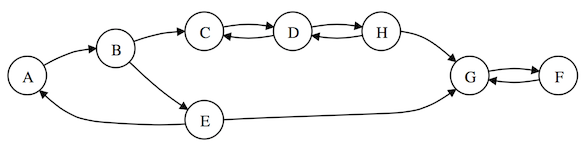
\includegraphics[width=0.5\textwidth]{./tarjan.png}
          \label{fig:}
        \end{figure}

      \item[Undirected]
        Diese sind analog zu denen in der Vorlesung.

        \begin{figure}[h!]
          \centering
          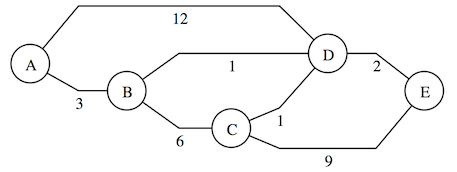
\includegraphics[width=0.5\textwidth]{prim-input.png}
          \label{fig:input}
        \end{figure}

      \item[Multigraph]
        Hier k\"onnen mehrere Kanten zwei gleiche Knoten verbinden. Nicht
        zu verwechseln mit einem ``Hypergraphen'', bei dem eine Kante mehrere
        Knoten verbinden kann.

        \begin{figure}[h!]
          \centering
          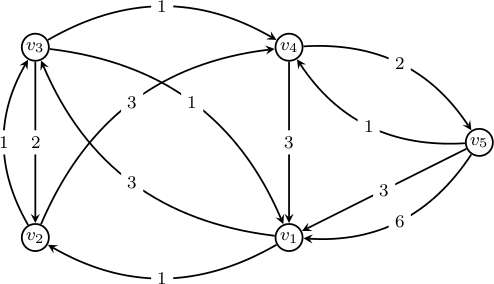
\includegraphics[width=0.5\textwidth]{weighted-multigraph.png}
          \label{fig:multigraph}
        \end{figure}

      \item[Compound]
        Diese sind wie B\"aume mit Wurzeln. Es l\"asst sich eine Kind-Elternteil
        Hirarchie auf den Knoten beschreiben.

        \begin{figure}[h!]
          \centering
          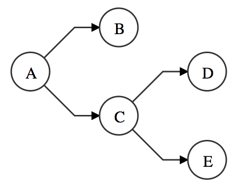
\includegraphics[width=0.3\textwidth]{preorder.png}
          \label{fig:preorder}
        \end{figure}
        
        
        \end{description}
\newpage

      \item \emph{Der Tarjan Algorithmus} \\
        Das Ziel dieses Algorithmus ist es, die Starken zusammenhangskomponenten
        eines gerichteten Graphen zu bestimmen.


\end{enumerate} 


\end{document}
